\documentclass{article}

% content/resources/templates/preamble.tex
\usepackage[margin=0.6in]{geometry}
\author{Milav Dabgar}
\usepackage{amsmath,amssymb,amsthm}
\usepackage{booktabs}
\usepackage{multirow}
\usepackage{xcolor}
\usepackage{tcolorbox}
\tcbuselibrary{breakable,skins}
\usepackage[colorlinks=true,linkcolor=blue]{hyperref}
\usepackage{titlesec}
\usepackage{enumitem}
\usepackage{tikz}
\usepackage{pgfplots}
\usepackage{circuitikz}
\usepackage[version=4]{mhchem}
\usepackage{longtable}
\usepackage{array}
\usepackage{float}
\usepackage{caption}
\usepackage{listings}

\lstset{
  basicstyle=\small\ttfamily,
  breaklines=true,
  breakatwhitespace=false,
  postbreak=\mbox{\textcolor{red}{$\hookrightarrow$}\space},
  float=false,
  numbers=left,
  numberstyle=\tiny\color{gray},
  numbersep=10pt,
  xleftmargin=2em,
  keywordstyle=\color{blue},
  commentstyle=\color{green!60!black},
  stringstyle=\color{purple},
  backgroundcolor=\color{gray!5},
  showstringspaces=false,
  tabsize=2,
  captionpos=b,
  keepspaces=true,
  columns=flexible
}

\pgfplotsset{compat=1.18}
\usetikzlibrary{shapes,arrows,positioning,calc,patterns,decorations.pathmorphing,decorations.markings,arrows.meta}

% Color scheme
\definecolor{headcolor}{RGB}{0,102,204}
\definecolor{keycolor}{RGB}{220,20,60}
\definecolor{solutioncolor}{RGB}{34,139,34}
\definecolor{mnemoniccolor}{RGB}{148,0,211}
\definecolor{codecolor}{RGB}{0,0,100}

% Spacing
\setlength{\parskip}{3pt}
\setlist[itemize]{nosep}
\setlist[enumerate]{nosep}

% Title formatting
\titleformat{\section}{\Large\bfseries\color{headcolor}}{\thesection}{1em}{}
\titleformat{\subsection}{\large\bfseries\color{headcolor}}{\thesubsection}{1em}{}

% Pandoc tightlist compatibility
\providecommand{\tightlist}{%
  \setlength{\itemsep}{0pt}\setlength{\parskip}{0pt}}

% Pandoc longtable compatibility
\newcounter{none}
\def\thenone{}


% content/resources/templates/english-boxes.tex

% Custom environments
\newtcolorbox{solutionbox}{
 breakable,
 enhanced,
 colback=solutioncolor!5!white,
 colframe=solutioncolor!75!black,
 fonttitle=\bfseries,
 title=Solution
}

\newtcolorbox{solutionboxnobreak}{
 colback=solutioncolor!5!white,
 colframe=solutioncolor!75!black,
 fonttitle=\bfseries,
 title=Solution
}

\newtcolorbox{keyformula}{
 breakable,
 enhanced,
 colback=keycolor!5!white,
 colframe=keycolor!75!black,
 fonttitle=\bfseries,
 title=Key Formula
}

\newtcolorbox{mnemonicboxenv}{
 breakable,
 enhanced,
 colback=mnemoniccolor!5!white,
 colframe=mnemoniccolor!75!black,
 fonttitle=\bfseries,
 title=Mnemonic
}

\newcommand{\mnemonicbox}[1]{%
  \begin{mnemonicboxenv}
    #1
  \end{mnemonicboxenv}
}


% Custom commands for GTU solutions
% This file defines semantic commands for consistent formatting

% Question command with automatic formatting
\newcommand{\question}[2]{%
  \section*{Question #1}%
  \textbf{#2}%
}

% OR question variant
\newcommand{\questionor}[2]{%
  \section*{Question #1 OR}%
  \textbf{#2}%
}

% Proper table environment with caption
\newenvironment{answertable}[1]{%
  \begin{table}[htbp]
  \centering
  \caption{#1}
}{%
  \end{table}
}

% Proper figure environment for diagrams
\newenvironment{answerdiagram}[1]{%
  \begin{figure}[htbp]
  \centering
  \caption{#1}
}{%
  \end{figure}
}

% Semantic markup for key terms
\newcommand{\keyword}[1]{\textbf{#1}}
\newcommand{\code}[1]{\texttt{#1}}
\newcommand{\classname}[1]{\texttt{#1}}
\newcommand{\methodname}[1]{\texttt{#1}}

% Proper quotation marks
\newcommand{\mnemonic}[1]{``#1''}


\title{Communication Engineering (1333201) - Summer 2025 Solution}
\date{May 09, 2025}

\begin{document}
\maketitle

\questionmarks{1(a)}{3}{Define AM, FM and PM.}

\begin{solutionbox}
\textbf{Answer}:

\begin{center}
\captionof{table}{Modulation Types Definition}
\begin{tabulary}{\linewidth}{|L|L|}
\hline
\textbf{Modulation Type} & \textbf{Definition} \\
\hline
\textbf{AM (Amplitude Modulation)} & Process where amplitude of carrier signal varies in accordance with the instantaneous amplitude of the message signal \\
\hline
\textbf{FM (Frequency Modulation)} & Process where frequency of carrier signal varies in accordance with the instantaneous amplitude of the message signal \\
\hline
\textbf{PM (Phase Modulation)} & Process where phase of carrier signal varies in accordance with the instantaneous amplitude of the message signal \\
\hline
\end{tabulary}
\end{center}
\end{solutionbox}

\begin{mnemonicbox}
"AFaP" - "Amplitude, Frequency and Phase" are the three parameters changed during modulation.
\end{mnemonicbox}

\questionmarks{1(b)}{4}{Explain block diagram of communication system.}

\begin{solutionbox}
\textbf{Answer}:

\begin{center}
\begin{tikzpicture}[node distance=2.5cm, auto, >=latex, thick]
    % Nodes
    \node [gtu block] (source) {Information\\Source};
    \node [gtu block, right of=source] (tx) {Transmitter};
    \node [gtu block, right of=tx] (channel) {Channel};
    \node [gtu block, right of=channel] (rx) {Receiver};
    \node [gtu block, right of=rx] (dest) {Destination};
    \node [gtu block, below of=channel, node distance=2cm] (noise) {Noise Source};

    % Arrows
    \draw [gtu arrow] (source) -- (tx);
    \draw [gtu arrow] (tx) -- (channel);
    \draw [gtu arrow] (channel) -- (rx);
    \draw [gtu arrow] (rx) -- (dest);
    \draw [gtu arrow] (noise) -- (channel);
\end{tikzpicture}
\captionof{figure}{Communication System}
\end{center}

\textbf{Components of Communication System:}
\begin{itemize}
    \item \textbf{Information Source}: Produces message to be communicated
    \item \textbf{Transmitter}: Converts message to signals suitable for transmission
    \item \textbf{Channel}: Medium through which signals travel
    \item \textbf{Receiver}: Extracts original message from received signal
    \item \textbf{Destination}: Person/device for whom message is intended
    \item \textbf{Noise Source}: Unwanted signals that interfere with transmitted signal
\end{itemize}
\end{solutionbox}

\begin{mnemonicbox}
"I Transmit Communication Reliably Despite Noise"
\end{mnemonicbox}

\questionmarks{1(c)}{7}{Explain Amplitude modulation with waveform and derive voltage equation for modulated signal also Sketch the frequency spectrum of the DSBFC AM.}

\begin{solutionbox}
\textbf{Answer}:
Amplitude Modulation is the process where the amplitude of a high-frequency carrier wave varies according to the instantaneous value of the modulating signal.

\textbf{Waveform and Equation:}

\begin{center}
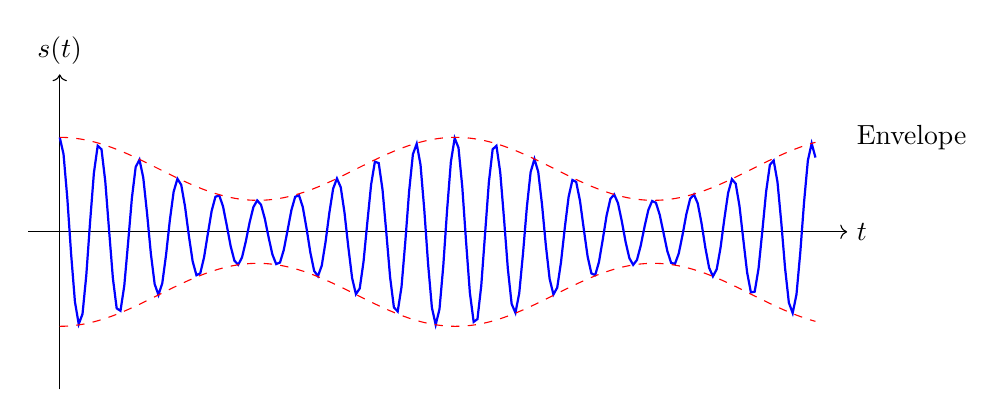
\begin{tikzpicture}[domain=0:12, samples=200, scale=0.8]
    \draw[->] (-0.5,0) -- (12.5,0) node[right] {$t$};
    \draw[->] (0,-2.5) -- (0,2.5) node[above] {$s(t)$};
    
    % AM Signal: (1 + 0.5cos(t)) * cos(10t)
    \draw[blue, thick] plot (\x, {(1 + 0.5*cos(\x r)) * cos(10*\x r)});
    \draw[red, dashed] plot (\x, {1 + 0.5*cos(\x r)});
    \draw[red, dashed] plot (\x, {-1 - 0.5*cos(\x r)});
    
    \node[right] at (12.5, 1.5) {Envelope};
\end{tikzpicture}
\captionof{figure}{AM Waveform}
\end{center}

\textbf{Derivation of AM equation:}
\begin{itemize}
    \item Carrier signal: $c(t) = A_c \cos(\omega_c t)$
    \item Modulating signal: $m(t) = A_m \cos(\omega_m t)$
    \item Modulation Index: $\mu = A_m/A_c$
    \item AM signal: $s(t) = A_c[1 + \mu \cdot \cos(\omega_m t)]\cos(\omega_c t)$
    \item Expanding: $s(t) = A_c \cdot \cos(\omega_c t) + \frac{\mu A_c}{2} \cos[(\omega_c+\omega_m)t] + \frac{\mu A_c}{2} \cos[(\omega_c-\omega_m)t]$
\end{itemize}

\textbf{DSBFC AM Frequency Spectrum:}

\begin{center}
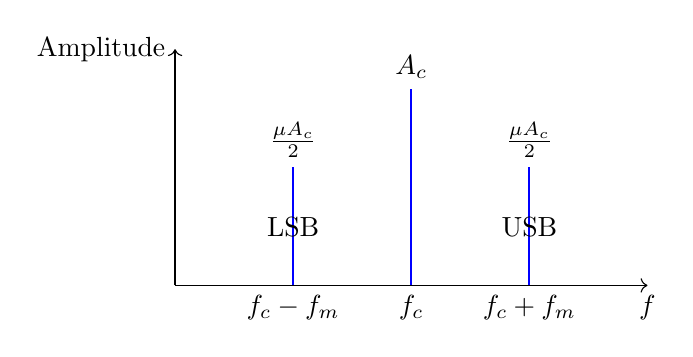
\begin{tikzpicture}[scale=1]
    \draw[->] (0,0) -- (6,0) node[below] {$f$};
    \draw[->] (0,0) -- (0,3) node[left] {Amplitude};
    
    % Carrier
    \draw[thick, blue] (3,0) -- (3,2.5);
    \node[above] at (3,2.5) {$A_c$};
    \node[below] at (3,0) {$f_c$};
    
    % LSB
    \draw[thick, blue] (1.5,0) -- (1.5,1.5);
    \node[above] at (1.5,1.5) {$\frac{\mu A_c}{2}$};
    \node[below] at (1.5,0) {$f_c - f_m$};
    \node[above] at (1.5, 0.5) {LSB};

    % USB
    \draw[thick, blue] (4.5,0) -- (4.5,1.5);
    \node[above] at (4.5,1.5) {$\frac{\mu A_c}{2}$};
    \node[below] at (4.5,0) {$f_c + f_m$};
    \node[above] at (4.5, 0.5) {USB};
\end{tikzpicture}
\captionof{figure}{DSBFC AM Frequency Spectrum}
\end{center}

\textbf{Key Points:}
\begin{itemize}
    \item \textbf{LSB (Lower Sideband)}: Located at $f_c-f_m$
    \item \textbf{USB (Upper Sideband)}: Located at $f_c+f_m$
    \item \textbf{Bandwidth}: $2f_m$ (twice the highest modulating frequency)
\end{itemize}
\end{solutionbox}

\begin{mnemonicbox}
"CARrying Two SideBands" - DSBFC AM carries both sidebands.
\end{mnemonicbox}

\questionmarks{1(c) OR}{7}{Derive the equation for total power in AM, calculate percentage of power savings in DSBFC And SSBSC.}

\begin{solutionbox}
\textbf{Answer}:

\textbf{Total Power in AM:}
For AM signal $s(t) = A_c[1 + \mu \cdot \cos(\omega_m t)]\cos(\omega_c t)$:

\textbf{Power Calculation:}
\begin{itemize}
    \item Carrier Power: $P_c = A_c^2/2$
    \item Power in each sideband: $P_{USB} = P_{LSB} = P_c \cdot \mu^2/4$
    \item Total Sideband Power: $P_{USB} + P_{LSB} = P_c \cdot \mu^2/2$
    \item Total Power: $P_t = P_c + P_{USB} + P_{LSB} = P_c(1 + \mu^2/2)$
\end{itemize}

\textbf{Power Savings:}

\begin{center}
\captionof{table}{Power Savings}
\begin{tabulary}{\linewidth}{|L|L|L|}
\hline
\textbf{Modulation} & \textbf{Power Distribution} & \textbf{Power Savings} \\
\hline
\textbf{DSBFC AM} & Uses carrier + both sidebands & 0\% (reference) \\
\hline
\textbf{SSBSC AM} & Uses only one sideband, no carrier & $\frac{2 - \mu^2/2}{1 + \mu^2/2} \times 100\%$ \\
\hline
\end{tabulary}
\end{center}

For $\mu = 1$, SSBSC saves approximately 85\% power compared to DSBFC.
\end{solutionbox}

\begin{mnemonicbox}
"SSB Saves Power By Cutting Carrier"
\end{mnemonicbox}

\questionmarks{2(a)}{3}{Compare AM and FM.}

\begin{solutionbox}
\textbf{Answer}:

\begin{center}
\captionof{table}{Comparison of AM and FM}
\begin{tabulary}{\linewidth}{|L|L|L|}
\hline
\textbf{Parameter} & \textbf{AM} & \textbf{FM} \\
\hline
\textbf{Definition} & Amplitude of carrier varies with message signal & Frequency of carrier varies with message signal \\
\hline
\textbf{Bandwidth} & 2 $\times$ message frequency & 2 $\times$ ($\Delta f + f_m$) \\
\hline
\textbf{Noise Immunity} & Poor (noise affects amplitude) & Excellent (noise mainly affects amplitude) \\
\hline
\textbf{Power Efficiency} & Low (carrier contains most power) & High (all transmitted power contains information) \\
\hline
\textbf{Circuit Complexity} & Simple, inexpensive & Complex, expensive \\
\hline
\end{tabulary}
\end{center}
\end{solutionbox}

\begin{mnemonicbox}
"AM Needs Power, FM Fights Noise"
\end{mnemonicbox}

\questionmarks{2(b)}{4}{Draw and explain block diagram for envelope detector.}

\begin{solutionbox}
\textbf{Answer}:

\begin{center}
\begin{tikzpicture}[auto, >=latex, thick]
    \node (input) {AM Input};
    \node [right of=input, node distance=2cm] (diode) {};
    % Diode symbol
    \draw (diode) -- ++(1,0) coordinate (d1);
    \draw (d1) -- ++(0.5,0.5) -- ++(0,-1) -- ++(-0.5,0.5); 
    \draw (d1) ++(0.5,-0.5) -- ++(0,1);
    \draw (d1) ++(0.5,0) -- ++(1,0) coordinate (node1);
    
    % RC parallel
    \draw (node1) -- ++(0,-1.5) coordinate (c_top);
    \draw (c_top) to[C, l=C] ++(0,-1.5) coordinate (gnd);
    \draw (node1) -- ++(2,0) coordinate (node2);
    \draw (node2) -- ++(0,-1.5) coordinate (r_top);
    \draw (r_top) to[R, l=R] ++(0,-1.5) coordinate (gnd2);
    
    % Ground
    \node [ground] at (gnd) {};
    \node [ground] at (gnd2) {};
    
    % Output
    \draw (node2) -- ++(1.5,0) node[right] (output) {Output Signal};
    
    \node [above of=diode] {Diode};
\end{tikzpicture}
\captionof{figure}{Envelope Detector}
\end{center}

\textbf{Components of Envelope Detector:}
\begin{itemize}
    \item \textbf{Diode}: Rectifies the AM signal (allows current flow in one direction)
    \item \textbf{RC Circuit}: R and C values chosen such that:
    \begin{itemize}
        \item $RC \gg 1/f_c$ (to filter carrier frequency)
        \item $RC \ll 1/f_m$ (to follow the envelope)
    \end{itemize}
\end{itemize}

\textbf{Working:}
\begin{enumerate}
    \item Diode conducts during positive half-cycles of carrier
    \item Capacitor charges to peak value
    \item When input falls, capacitor discharges through resistor
    \item Output follows envelope of AM signal
\end{enumerate}
\end{solutionbox}

\begin{mnemonicbox}
"Detect, Rect, and Connect" - Detection through Rectification and RC connection.
\end{mnemonicbox}

\questionmarks{2(c)}{7}{Draw block diagram of FM radio receiver and explain working of each block.}

\begin{solutionbox}
\textbf{Answer}:

\begin{center}
\begin{tikzpicture}[node distance=2cm, auto, >=latex, thick, scale=0.8, transform shape]
    \node [gtu block] (ant) {Antenna};
    \node [gtu block, right of=ant, node distance=2.2cm] (rf) {RF Amp};
    \node [gtu block, right of=rf, node distance=2.2cm] (mix) {Mixer};
    \node [gtu block, below of=mix] (lo) {Local Osc};
    \node [gtu block, right of=mix, node distance=2.2cm] (if) {IF Amp};
    \node [gtu block, right of=if, node distance=2.2cm] (lim) {Limiter};
    \node [gtu block, right of=lim, node distance=2.2cm] (det) {FM Detector};
    \node [gtu block, right of=det, node distance=2.2cm] (af) {Audio Amp};
    \node [gtu block, right of=af, node distance=2.2cm] (spk) {Speaker};

    \draw [gtu arrow] (ant) -- (rf);
    \draw [gtu arrow] (rf) -- (mix);
    \draw [gtu arrow] (lo) -- (mix);
    \draw [gtu arrow] (mix) -- (if);
    \draw [gtu arrow] (if) -- (lim);
    \draw [gtu arrow] (lim) -- (det);
    \draw [gtu arrow] (det) -- (af);
    \draw [gtu arrow] (af) -- (spk);
\end{tikzpicture}
\captionof{figure}{FM Radio Receiver}
\end{center}

\textbf{Working of Each Block:}
\begin{itemize}
    \item \textbf{Antenna}: Receives FM broadcast signals (88-108 MHz)
    \item \textbf{RF Amplifier}: Amplifies weak RF signals, provides selectivity
    \item \textbf{Mixer \& Local Oscillator}: Converts RF to fixed IF (10.7 MHz) using heterodyning
    \item \textbf{IF Amplifier}: Provides most of receiver's gain and selectivity
    \item \textbf{Limiter}: Removes amplitude variations from FM signal
    \item \textbf{FM Detector}: Converts frequency variations to audio (uses ratio detector/PLL)
    \item \textbf{Audio Amplifier}: Amplifies recovered audio signal
    \item \textbf{Speaker}: Converts electrical signals to sound
\end{itemize}
\end{solutionbox}

\begin{mnemonicbox}
"Really Mighty Instruments Limit Frequency And Make Sound"
\end{mnemonicbox}

\questionmarks{2(a) OR}{3}{Define Sensitivity, Selectivity, Fidelity for radio receiver.}

\begin{solutionbox}
\textbf{Answer}:

\begin{center}
\captionof{table}{Receiver Characteristics}
\begin{tabulary}{\linewidth}{|L|L|}
\hline
\textbf{Parameter} & \textbf{Definition} \\
\hline
\textbf{Sensitivity} & Ability of receiver to amplify weak signals (measured in $\mu V$) \\
\hline
\textbf{Selectivity} & Ability to separate desired signal from adjacent signals \\
\hline
\textbf{Fidelity} & Ability to reproduce the original signal without distortion \\
\hline
\end{tabulary}
\end{center}
\end{solutionbox}

\begin{mnemonicbox}
"SSF" - "Select Signals Faithfully"
\end{mnemonicbox}

\questionmarks{2(b) OR}{4}{Explain ratio detector for FM.}

\begin{solutionbox}
\textbf{Answer}:

\begin{center}
\begin{tikzpicture}[auto, >=latex, thick]
    % Simplified representation
    \node [gtu block] (input) {FM Input / Transformer};
    \node [gtu block, right of=input, node distance=3.5cm] (diodes) {Diode Bridge};
    \node [gtu block, right of=diodes, node distance=3.5cm] (cap) {Large Cap ($10\mu F$)};
    \node [gtu block, right of=cap, node distance=3.5cm] (out) {Audio Output};

    \draw [gtu arrow] (input) -- (diodes);
    \draw [gtu arrow] (diodes) -- (cap);
    \draw [gtu arrow] (cap) -- (out);
\end{tikzpicture}
\captionof{figure}{Ratio Detector}
\end{center}

\textbf{Working of Ratio Detector:}
\begin{itemize}
    \item Uses balanced circuit with two diodes in series
    \item Large stabilizing capacitor keeps sum of voltages constant
    \item Output voltage is proportional to frequency deviation
    \item Inherently insensitive to amplitude variations (no limiter needed)
    \item Less susceptible to impulse noise than discriminator
\end{itemize}
\end{solutionbox}

\begin{mnemonicbox}
"RADS" - "Ratio And Diodes Stabilize"
\end{mnemonicbox}

\questionmarks{2(c) OR}{7}{Draw block diagram of AM radio receiver and explain working of each block.}

\begin{solutionbox}
\textbf{Answer}:

\begin{center}
\begin{tikzpicture}[node distance=2cm, auto, >=latex, thick, scale=0.8, transform shape]
    \node [gtu block] (ant) {Antenna};
    \node [gtu block, right of=ant, node distance=2.2cm] (rf) {RF Amp};
    \node [gtu block, right of=rf, node distance=2.2cm] (mix) {Mixer};
    \node [gtu block, below of=mix] (lo) {Local Osc};
    \node [gtu block, right of=mix, node distance=2.2cm] (if) {IF Amp};
    \node [gtu block, right of=if, node distance=2.2cm] (det) {Detector};
    \node [gtu block, below of=det] (agc) {AGC};
    \node [gtu block, right of=det, node distance=2.2cm] (af) {Audio Amp};
    \node [gtu block, right of=af, node distance=2.2cm] (spk) {Speaker};

    \draw [gtu arrow] (ant) -- (rf);
    \draw [gtu arrow] (rf) -- (mix);
    \draw [gtu arrow] (lo) -- (mix);
    \draw [gtu arrow] (mix) -- (if);
    \draw [gtu arrow] (if) -- (det);
    \draw [gtu arrow] (det) -- (af);
    \draw [gtu arrow] (af) -- (spk);
    
    % AGC feedback
    \draw [gtu arrow] (det) -- (agc);
    \draw [gtu arrow] (agc) -| (if);
    \draw [gtu arrow] (agc) -| (rf);
\end{tikzpicture}
\captionof{figure}{AM Radio Receiver}
\end{center}

\textbf{Working of Each Block:}
\begin{itemize}
    \item \textbf{Antenna}: Intercepts AM broadcast signals (535-1605 kHz)
    \item \textbf{RF Amplifier}: Amplifies weak RF signals with good SNR
    \item \textbf{Mixer \& Local Oscillator}: Converts RF to fixed IF (455 kHz)
    \item \textbf{IF Amplifier}: Provides most gain and selectivity at 455 kHz
    \item \textbf{Detector}: Extracts audio from AM signal (envelope detector)
    \item \textbf{AGC (Automatic Gain Control)}: Maintains constant output level
    \item \textbf{Audio Amplifier}: Boosts detected audio to drive speaker
    \item \textbf{Speaker}: Converts electrical signals to sound waves
\end{itemize}
\end{solutionbox}

\begin{mnemonicbox}
"ARMIDAS" - "Amplify, Mix, IF, Detect, Audio, Speak"
\end{mnemonicbox}

\questionmarks{3(a)}{3}{Describe the Nyquist criteria.}

\begin{solutionbox}
\textbf{Answer}:

\textbf{Nyquist Criteria}: To accurately reconstruct a signal from its samples, the sampling frequency ($f_s$) must be at least twice the highest frequency ($f_{max}$) present in the signal.

\begin{center}
\captionof{table}{Nyquist Criteria}
\begin{tabulary}{\linewidth}{|L|L|L|}
\hline
\textbf{Parameter} & \textbf{Formula} & \textbf{Description} \\
\hline
\textbf{Nyquist Rate} & $f_s \ge 2f_{max}$ & Minimum sampling rate required \\
\hline
\textbf{Nyquist Interval} & $T_s \le 1/2f_{max}$ & Maximum time between samples \\
\hline
\end{tabulary}
\end{center}

\textbf{Consequence if violated}: Aliasing occurs - higher frequencies appear as lower frequencies in sampled signal.
\end{solutionbox}

\begin{mnemonicbox}
"Sample Double to Dodge Aliasing"
\end{mnemonicbox}

\questionmarks{3(b)}{4}{Explain Sample and hold Circuit with Waveform.}

\begin{solutionbox}
\textbf{Answer}:

\begin{center}
\begin{tikzpicture}[auto, >=latex, thick]
    \node (input) {Analog Input};
    \node [draw, rectangle, right of=input, node distance=2.5cm] (switch) {Switch};
    \node [above of=switch] (clock) {Clock};
    \node [right of=switch, node distance=2cm] (node1) {};
    \node [below of=node1] (cap) {Capacitor};
    \node [gtu block, right of=node1, node distance=2cm] (buffer) {Buffer};
    \node [right of=buffer, node distance=2cm] (output) {Output};

    \draw [gtu arrow] (input) -- (switch);
    \draw [gtu arrow] (clock) -- (switch);
    \draw [gtu arrow] (switch) -- (buffer);
    \draw [gtu arrow] (buffer) -- (output);
    \draw (node1) -- (cap);
    \node [ground, below of=cap, node distance=0.8cm] (gnd) {};
    \draw (cap) -- (gnd);
\end{tikzpicture}
\captionof{figure}{Sample and Hold Circuit}
\end{center}

\textbf{Sample and Hold Circuit Operation:}
\begin{itemize}
    \item \textbf{Electronic Switch}: Closes briefly during sampling
    \item \textbf{Capacitor}: Stores sampled voltage
    \item \textbf{Buffer Amplifier}: Provides high input impedance and low output impedance
\end{itemize}

\textbf{Waveform:}
\begin{center}
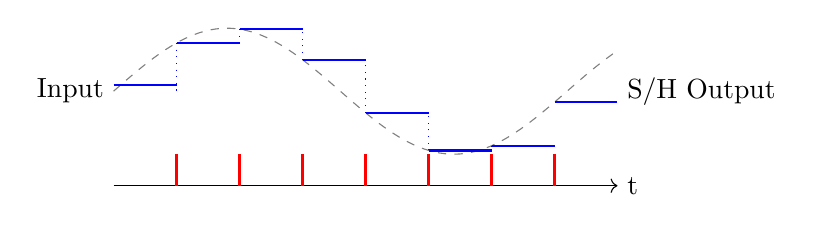
\begin{tikzpicture}[scale=0.8]
    \draw[->] (0,0) -- (8,0) node[right] {t};
    % Analog Input
    \draw[gray, dashed] plot[domain=0:8, samples=100] (\x, {1.5 + 1*sin(\x*50)});
    \node[left] at (0, 1.5) {Input};
    
    % Clock (Switch closing)
    \foreach \x in {1,2,3,4,5,6,7} {
        \draw[thick, red] (\x, 0) -- (\x, 0.5);
    }
    
    % Output (Step)
    \draw[blue, thick] (0, 1.6) -- (1, 1.6); % Start
    \foreach \x in {1,2,3,4,5,6} {
        \draw[blue, thick] (\x, {1.5 + 1*sin(\x*50)}) -- (\x+1, {1.5 + 1*sin(\x*50)});
        \draw[blue, dotted] (\x, {1.5 + 1*sin(\x*50)}) -- (\x, {1.5 + 1*sin((\x-1)*50)}); 
    }
    \draw[blue, thick] (7, {1.5 + 1*sin(350)}) -- (8, {1.5 + 1*sin(350)});
    
    \node[right] at (8, 1.5) {S/H Output};
\end{tikzpicture}
\captionof{figure}{Sample and Hold Waveforms}
\end{center}

\textbf{Applications:}
\begin{itemize}
    \item Analog-to-Digital Conversion
    \item Data Acquisition Systems
    \item Pulse Amplitude Modulation
\end{itemize}
\end{solutionbox}

\begin{mnemonicbox}
"SCAB" - "Switch, Capacitor And Buffer"
\end{mnemonicbox}

\questionmarks{3(c)}{7}{Define quantization explain uniform and non-uniform quantization in details.}

\begin{solutionbox}
\textbf{Answer}:

\textbf{Quantization}: Process of mapping a large set of input values to a smaller set of discrete output values.

\begin{center}
\begin{tikzpicture}[auto, >=latex, thick]
    \node [gtu block] (cont) {Continuous\\Amplitude};
    \node [gtu block, right of=cont, node distance=3.5cm] (disc) {Discrete\\Amplitude};
    \node [gtu block, right of=disc, node distance=3.5cm] (dig) {Digital\\Code};
    \draw [gtu arrow] (cont) -- (disc);
    \draw [gtu arrow] (disc) -- (dig);
\end{tikzpicture}
\captionof{figure}{Quantization Process}
\end{center}

\textbf{Uniform Quantization vs Non-uniform Quantization:}

\begin{center}
\captionof{table}{Comparison of Quantization Types}
\begin{tabulary}{\linewidth}{|L|L|L|}
\hline
\textbf{Parameter} & \textbf{Uniform Quantization} & \textbf{Non-uniform Quantization} \\
\hline
\textbf{Step Size} & Equal throughout range & Varies (smaller for small signals) \\
\hline
\textbf{Characteristic} & Linear & Non-linear (logarithmic/exponential) \\
\hline
\textbf{SNR} & Poor for small signals & Better for small signals \\
\hline
\textbf{Implementation} & Simple & Complex (companding required) \\
\hline
\textbf{Applications} & Simple signals, images & Speech, audio ($\mu$-law, A-law) \\
\hline
\end{tabulary}
\end{center}

\textbf{Quantization Error:}
\begin{itemize}
    \item Difference between original and quantized signal
    \item Maximum error = $\pm Q/2$ (where Q is quantization step size)
    \item Appears as quantization noise in reconstructed signal
\end{itemize}
\end{solutionbox}

\begin{mnemonicbox}
"UNIQ" - "UNIform has equal steps, non-uniform Quiets noise"
\end{mnemonicbox}

\questionmarks{3(a) OR}{3}{Explain aliasing error and how to overcome it.}

\begin{solutionbox}
\textbf{Answer}:

\textbf{Aliasing Error}: Distortion that occurs when a signal is sampled at a rate lower than twice its highest frequency component.

\begin{center}
\begin{tikzpicture}[node distance=2cm, auto, >=latex]
    \node [gtu block] (alias) {Aliasing Error};
    \node [right of=alias, node distance=4cm, text width=4cm, align=left] (effects) {1. Original high freq appears as false low freq\\2. Irreversible distortion};
    \draw [->, thick] (alias) -- (effects);
\end{tikzpicture}
\end{center}

\textbf{How to Overcome Aliasing:}
\begin{itemize}
    \item Use anti-aliasing filter (low-pass) before sampling
    \item Increase sampling rate above Nyquist rate ($f_s > 2f_{max}$)
    \item Bandlimit the input signal before sampling
\end{itemize}
\end{solutionbox}

\begin{mnemonicbox}
"ALIAS" - "Avoid Low sampling by Increasing And Screening"
\end{mnemonicbox}

\questionmarks{3(b) OR}{4}{Draw following signal in time domain and frequency domain: 1) Sawtooth signal 2) Pulse signal.}

\begin{solutionbox}
\textbf{Answer}:

\textbf{1. Sawtooth Signal:}
\begin{center}
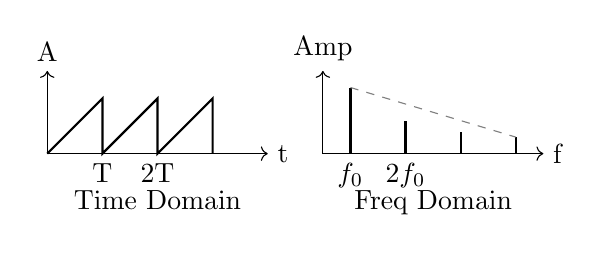
\begin{tikzpicture}[scale=0.7]
    % Time
    \begin{scope}
        \draw[->] (0,0) -- (4,0) node[right] {t};
        \draw[->] (0,0) -- (0,1.5) node[above] {A};
        \draw[thick] (0,0) -- (1,1) -- (1,0) -- (2,1) -- (2,0) -- (3,1) -- (3,0);
        \node[below] at (1,0) {T};
        \node[below] at (2,0) {2T};
        \node[below] at (2,-0.5) {Time Domain};
    \end{scope}
    
    % Freq
    \begin{scope}[xshift=5cm]
        \draw[->] (0,0) -- (4,0) node[right] {f};
        \draw[->] (0,0) -- (0,1.5) node[above] {Amp};
        \draw[thick] (0.5,0) -- (0.5,1.2);
        \draw[thick] (1.5,0) -- (1.5,0.6);
        \draw[thick] (2.5,0) -- (2.5,0.4);
        \draw[thick] (3.5,0) -- (3.5,0.3);
        
        \draw[dashed, gray] (0.5,1.2) -- (3.5,0.3);
        
        \node[below] at (0.5,0) {$f_0$};
        \node[below] at (1.5,0) {$2f_0$};
        \node[below] at (2,-0.5) {Freq Domain};
    \end{scope}
\end{tikzpicture}
\captionof{figure}{Sawtooth Signal}
\end{center}

\textbf{2. Pulse Signal:}
\begin{center}
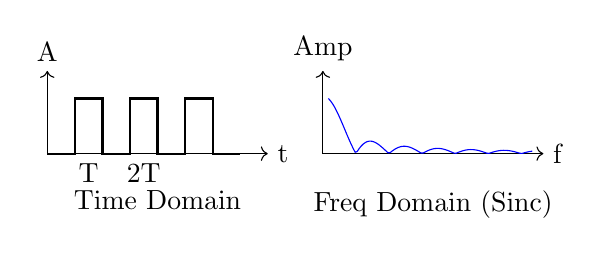
\begin{tikzpicture}[scale=0.7]
    % Time
    \begin{scope}
        \draw[->] (0,0) -- (4,0) node[right] {t};
        \draw[->] (0,0) -- (0,1.5) node[above] {A};
        \draw[thick] (0,0) -- (0.5,0) -- (0.5,1) -- (1,1) -- (1,0) 
                     -- (1.5,0) -- (1.5,1) -- (2,1) -- (2,0)
                     -- (2.5,0) -- (2.5,1) -- (3,1) -- (3,0) -- (3.5,0);
        \node[below] at (0.75,0) {T};
        \node[below] at (1.75,0) {2T};
        \node[below] at (2,-0.5) {Time Domain};
    \end{scope}
    
    % Freq
    \begin{scope}[xshift=5cm]
        \draw[->] (0,0) -- (4,0) node[right] {f};
        \draw[->] (0,0) -- (0,1.5) node[above] {Amp};
        
        \draw[domain=0.1:3.8, samples=100, blue] plot (\x, {abs(sin(300*\x)/(5*\x))});
        
        \node[below] at (2,-0.5) {Freq Domain (Sinc)};
    \end{scope}
\end{tikzpicture}
\captionof{figure}{Pulse Signal}
\end{center}
\end{solutionbox}

\begin{mnemonicbox}
"STPF" - "SawTooth slopes down, Pulse has sinc Function"
\end{mnemonicbox}

\questionmarks{3(c) OR}{7}{Compare PAM, PWM and PPM with waveform.}

\begin{solutionbox}
\textbf{Answer}:

\begin{center}
\captionof{table}{Comparison of Pulse Modulation}
\begin{tabulary}{\linewidth}{|L|L|L|L|}
\hline
\textbf{Parameter} & \textbf{PAM} & \textbf{PWM} & \textbf{PPM} \\
\hline
\textbf{Full Form} & Pulse Amplitude Modulation & Pulse Width Modulation & Pulse Position Modulation \\
\hline
\textbf{Parameter Varied} & Amplitude of pulses & Width/duration of pulses & Position/timing of pulses \\
\hline
\textbf{Noise Immunity} & Poor & Good & Excellent \\
\hline
\textbf{Bandwidth} & Lower & Higher & Highest \\
\hline
\textbf{Power Efficiency} & Low & Medium & High \\
\hline
\textbf{Demodulation} & Simple & Moderate & Complex \\
\hline
\end{tabulary}
\end{center}

\textbf{Waveforms:}
\begin{center}
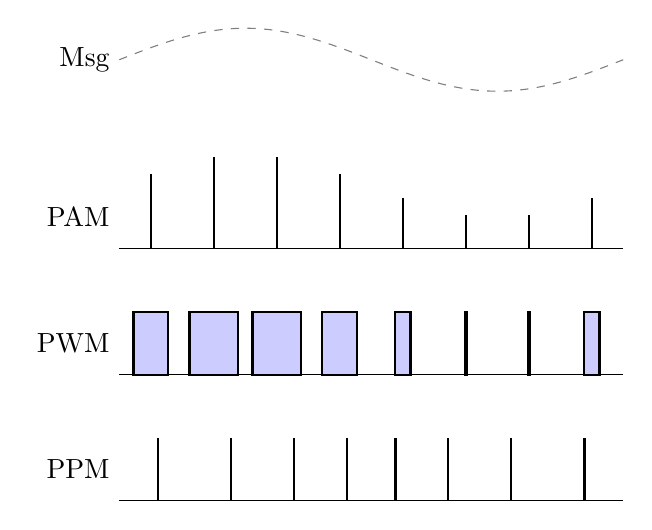
\begin{tikzpicture}[scale=0.8]
    % Message
    \draw[gray, dashed] plot[domain=0:8, samples=100] (\x, {1 + 0.5*sin(180*\x/4)});
    \node[left] at (0,1) {Msg};

    % PAM
    \begin{scope}[yshift=-2cm]
        \foreach \x in {0.5, 1.5, ..., 7.5} {
            \draw[thick] (\x,0) -- (\x, {1 + 0.5*sin(180*\x/4)});
        }
        \draw (0,0) -- (8,0);
        \node[left] at (0,0.5) {PAM};
    \end{scope}

    % PWM
    \begin{scope}[yshift=-4cm]
        \foreach \x in {0.5, 1.5, ..., 7.5} {
            \pgfmathsetmacro{\w}{0.2 + 0.2*sin(180*\x/4)}
            \draw[thick, fill=blue!20] (\x-\w, 0) rectangle (\x+\w, 1);
        }
        \draw (0,0) -- (8,0);
        \node[left] at (0,0.5) {PWM};
    \end{scope}

    % PPM
    \begin{scope}[yshift=-6cm]
        \foreach \x in {0.5, 1.5, ..., 7.5} {
             \pgfmathsetmacro{\s}{0.3*sin(180*\x/4)}
            \draw[thick] (\x+\s, 0) -- (\x+\s, 1);
        }
        \draw (0,0) -- (8,0);
        \node[left] at (0,0.5) {PPM};
    \end{scope}
\end{tikzpicture}
\captionof{figure}{Pulse Modulation Waveforms}
\end{center}
\end{solutionbox}

\begin{mnemonicbox}
"APP" - "Amplitude, Pulse-width, Position"
\end{mnemonicbox}

\questionmarks{4(a)}{3}{Explain Space wave propagation.}

\begin{solutionbox}
\textbf{Answer}:

\textbf{Space Wave Propagation}: Mode where radio waves travel through lower atmosphere (troposphere) directly or via ground reflection.

\begin{center}
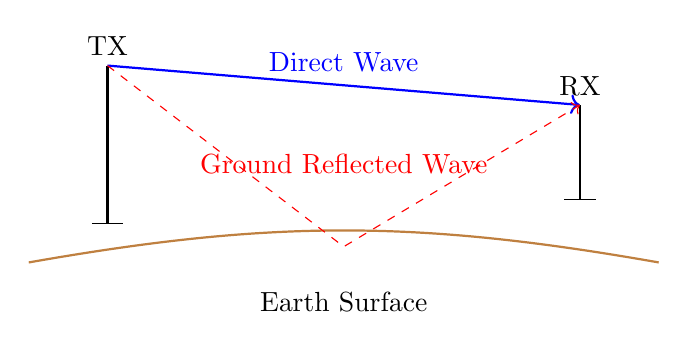
\begin{tikzpicture}[scale=1]
    % Ground
    \draw[thick, brown] (-4,0) to[out=10, in=170] (4,0);
    \node at (0,-0.5) {Earth Surface};
    
    % TX Tower
    \draw[thick] (-3,0.5) -- (-3,2.5);
    \draw (-3.2, 0.5) -- (-2.8, 0.5);
    \node[above] at (-3,2.5) {TX};
    
    % RX Tower
    \draw[thick] (3,0.8) -- (3,2);
    \draw (2.8, 0.8) -- (3.2, 0.8);
    \node[above] at (3,2) {RX};
    
    % Direct Wave
    \draw[blue, thick, ->] (-3,2.5) -- (3,2);
    \node[above, blue] at (0,2.3) {Direct Wave};
    
    % Reflected Wave
    \draw[red, dashed, ->] (-3,2.5) -- (0,0.2) -- (3,2);
    \node[below, red] at (0,1.5) {Ground Reflected Wave};
\end{tikzpicture}
\captionof{figure}{Space Wave Propagation}
\end{center}

\textbf{Characteristics:}
\begin{itemize}
    \item Frequency Range: VHF, UHF (30 MHz - 3 GHz)
    \item Limited to line-of-sight distance
    \item Range = $4.12(\sqrt{h_1} + \sqrt{h_2})$ km (where $h_1, h_2$ in meters)
    \item Affected by terrain, buildings, and atmospheric conditions
\end{itemize}
\end{solutionbox}

\begin{mnemonicbox}
"See Straight" - Space waves travel in straight lines.
\end{mnemonicbox}

\questionmarks{4(b)}{4}{Explain working of differential PCM transmitter.}

\begin{solutionbox}
\textbf{Answer}:

\begin{center}
\begin{tikzpicture}[auto, >=latex, thick]
    \node (input) {$x(nT)$};
    \node [draw, circle, right of=input, node distance=1.5cm] (sub) {$\Sigma$};
    \node [gtu block, right of=sub, node distance=2.5cm] (quant) {Quantizer};
    \node [gtu block, right of=quant, node distance=3cm] (enc) {Encoder};
    \node [right of=enc, node distance=2cm] (out) {DPCM};
    
    \node [draw, circle, below of=quant, node distance=2.5cm] (adder) {$\Sigma$};
    \node [gtu block, left of=adder, node distance=3cm] (pred) {Predictor};
    
    \draw [gtu arrow] (input) -- node[pos=0.9] {$+$} (sub);
    \draw [gtu arrow] (sub) -- node {$e(nT)$} (quant);
    \draw [gtu arrow] (quant) -- node {$e_q(nT)$} (enc);
    \draw [gtu arrow] (enc) -- (out);
    
    % Feedback path
    \draw [gtu arrow] (quant) -- (adder);
    \draw [gtu arrow] (adder) -- node {$x_q(nT)$} (pred);
    \draw [gtu arrow] (pred) -| node[near end] {$-$} node[midway, above] {$\hat{x}(nT)$} (sub);
    \draw [gtu arrow] (pred) -- (adder);
    
\end{tikzpicture}
\captionof{figure}{DPCM Transmitter}
\end{center}

\textbf{DPCM Transmitter Working:}
\begin{itemize}
    \item \textbf{Predictor}: Estimates current sample based on previous samples
    \item \textbf{Subtractor}: Calculates difference between actual and predicted value
    \item \textbf{Quantizer}: Converts difference signal to discrete levels
    \item \textbf{Encoder}: Converts quantized values to binary code
    \item \textbf{Feedback Loop}: Reconstructs signal exactly as receiver will see it
\end{itemize}

\textbf{Advantage}: Only difference signal is transmitted, requiring fewer bits.
\end{solutionbox}

\begin{mnemonicbox}
"Predict Difference Encode"
\end{mnemonicbox}

\questionmarks{4(c)}{7}{Explain delta modulator in details also explain slop overload noise and granular noise.}

\begin{solutionbox}
\textbf{Answer}:

\textbf{Delta Modulation (DM)}: Simplest form of differential PCM where difference signal is encoded with 1 bit.

\begin{center}
\begin{tikzpicture}[auto, >=latex, thick]
    \node (input) {$x(t)$};
    \node [draw, circle, right of=input, node distance=1.5cm] (sub) {$\Sigma$};
    \node [gtu block, right of=sub, node distance=2.5cm] (comp) {Comparator};
    \node [gtu block, right of=comp, node distance=2.5cm] (sample) {Sampler};
    \node [right of=sample, node distance=2cm] (out) {DM Out};
    
    \node [gtu block, below of=comp, node distance=2cm] (int) {Integrator};
    
    \draw [gtu arrow] (input) -- (sub);
    \draw [gtu arrow] (sub) -- (comp);
    \draw [gtu arrow] (comp) -- (sample);
    \draw [gtu arrow] (sample) -- (out);
    
    \draw [gtu arrow] (sample) |- (int);
    \draw [gtu arrow] (int) -| node[near end] {$-$} (sub);
\end{tikzpicture}
\captionof{figure}{Delta Modulator}
\end{center}

\textbf{Working Principle:}
\begin{itemize}
    \item Compares input signal with integrated version of previous output
    \item If input > integrated value: Transmit 1
    \item If input < integrated value: Transmit 0
    \item Step size ($\delta$) is fixed
\end{itemize}

\textbf{Noise in Delta Modulation:}

\begin{center}
\captionof{table}{Noise in Delta Modulation}
\begin{tabulary}{\linewidth}{|L|L|L|}
\hline
\textbf{Noise Type} & \textbf{Cause} & \textbf{Remedy} \\
\hline
\textbf{Slope Overload Noise} & Input signal changes faster than $\delta$ can track & Increase step size or sampling frequency \\
\hline
\textbf{Granular Noise} & Step size is too large for slowly varying signals & Decrease step size \\
\hline
\end{tabulary}
\end{center}
\end{solutionbox}

\begin{mnemonicbox}
"Slog" - "Slope and Granular in DM"
\end{mnemonicbox}

\questionmarks{4(a) OR}{3}{Explain Ground wave propagation.}

\begin{solutionbox}
\textbf{Answer}:

\textbf{Ground Wave Propagation}: Radio wave propagation that follows the curvature of the earth.

\begin{center}
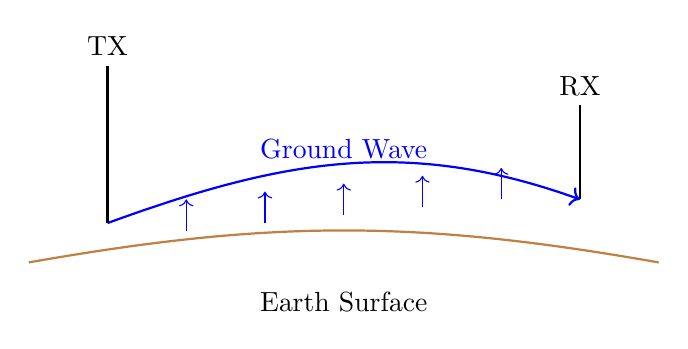
\begin{tikzpicture}[scale=1]
    % Ground
    \draw[thick, brown] (-4,0) to[out=10, in=170] (4,0);
    \node at (0,-0.5) {Earth Surface};
    
    % TX Tower
    \draw[thick] (-3,0.5) -- (-3,2.5);
    \node[above] at (-3,2.5) {TX};
    
    % RX Tower
    \draw[thick] (3,0.8) -- (3,2);
    \node[above] at (3,2) {RX};
    
    % Ground Wave
    \draw[blue, thick, ->] (-3,0.5) to[out=20, in=160] (3,0.8);
    \node[above, blue] at (0,1.2) {Ground Wave};
    
    % Vertical Polarization lines
    \foreach \x in {-2, -1, 0, 1, 2} {
        \draw[blue, ->] (\x, {0.6 + 0.1*\x}) -- (\x, {1.0 + 0.1*\x});
    }
\end{tikzpicture}
\captionof{figure}{Ground Wave Propagation}
\end{center}

\textbf{Characteristics:}
\begin{itemize}
    \item Frequency Range: LF, MF (30 kHz - 3 MHz)
    \item Propagates along earth's surface (vertically polarized)
    \item Range depends on tx power, ground conductivity, frequency
    \item Signal strength decreases with distance and frequency
    \item Used for AM broadcasting, marine communication
\end{itemize}
\end{solutionbox}

\begin{mnemonicbox}
"Ground Hugger" - Waves hug the ground.
\end{mnemonicbox}

\questionmarks{4(b) OR}{4}{Explain ADM Transmitter.}

\begin{solutionbox}
\textbf{Answer}:

\textbf{Adaptive Delta Modulation (ADM)}: Improved version of DM where step size varies according to signal characteristics.

\begin{center}
\begin{tikzpicture}[auto, >=latex, thick]
    \node (input) {$x(t)$};
    \node [draw, circle, right of=input, node distance=1.5cm] (sub) {$\Sigma$};
    \node [gtu block, right of=sub, node distance=2.5cm] (quant) {Quantizer};
    \node [right of=quant, node distance=2.5cm] (out) {ADM Out};
    
    \node [gtu block, below of=quant, node distance=2cm] (ctrl) {Step Size\\Control};
    \node [gtu block, left of=ctrl, node distance=2.5cm] (int) {Integrator};
    
    \draw [gtu arrow] (input) -- (sub);
    \draw [gtu arrow] (sub) -- (quant);
    \draw [gtu arrow] (quant) -- (out);
    
    \draw [gtu arrow] (quant) -- (ctrl);
    \draw [gtu arrow] (ctrl) -- (int);
    \draw [gtu arrow] (int) -| node[near end] {$-$} (sub);
\end{tikzpicture}
\captionof{figure}{ADM Transmitter}
\end{center}

\textbf{ADM Transmitter Working:}
\begin{itemize}
    \item \textbf{Basic Operation}: Similar to standard DM
    \item \textbf{Step Size Control}: Analyzes recent sequence of output bits
    \item \textbf{Adaptation Logic}:
    \begin{itemize}
        \item If consecutive bits are same: Increase step size
        \item If consecutive bits are alternate: Decrease step size
    \end{itemize}
\end{itemize}

\textbf{Advantages over DM:}
\begin{itemize}
    \item Reduces both slope overload and granular noise
    \item Better signal tracking
    \item Improved SNR
\end{itemize}
\end{solutionbox}

\begin{mnemonicbox}
"Adapt to Step" - Step size adapts to signal slope.
\end{mnemonicbox}

\questionmarks{4(c) OR}{7}{Explain block diagram of basic PCM-TDM System.}

\begin{solutionbox}
\textbf{Answer}:

\textbf{PCM-TDM System}: Combines Pulse Code Modulation with Time Division Multiplexing to transmit multiple digital signals over a single channel.

\begin{center}
\begin{tikzpicture}[node distance=2.5cm, auto, >=latex, thick, scale=0.8, transform shape]
    % Transmitter
    \node [gtu block] (in1) {Input 1};
    \node [gtu block, below of=in1, node distance=1.5cm] (in2) {Input 2};
    \node [gtu block, below of=in2, node distance=1.5cm] (in3) {Input n};
    
    \node [gtu block, right of=in2, node distance=3cm] (mux) {Multiplexer};
    \node [gtu block, right of=mux] (pcm) {PCM\\Encoder};
    \node [gtu block, right of=pcm] (tx) {TX};
    
    \draw [gtu arrow] (in1) -- (mux);
    \draw [gtu arrow] (in2) -- (mux);
    \draw [gtu arrow] (in3) -- (mux);
    \draw [gtu arrow] (mux) -- (pcm);
    \draw [gtu arrow] (pcm) -- (tx);
    
    % Channel
    \node [right of=tx, node distance=2cm] (ch) {};
    \draw [dashed] (tx) -- (ch);
    
    % Receiver
    \node [gtu block, right of=ch, node distance=2cm] (rx) {RX};
    \node [gtu block, right of=rx] (dec) {PCM\\Decoder};
    \node [gtu block, right of=dec] (demux) {Demul-\\tiplexer};
    
    \node [gtu block, right of=demux, node distance=3cm] (out2) {Output 2};
    \node [gtu block, above of=out2, node distance=1.5cm] (out1) {Output 1};
    \node [gtu block, below of=out2, node distance=1.5cm] (out3) {Output n};

    \draw [dashed] (ch) -- (rx);
    \draw [gtu arrow] (rx) -- (dec);
    \draw [gtu arrow] (dec) -- (demux);
    \draw [gtu arrow] (demux) -- (out1);
    \draw [gtu arrow] (demux) -- (out2);
    \draw [gtu arrow] (demux) -- (out3);
\end{tikzpicture}
\captionof{figure}{PCM-TDM System Block Diagram}
\end{center}

\textbf{PCM-TDM System Working:}
\begin{itemize}
    \item \textbf{Transmitter}:
    \begin{itemize}
        \item Multiple analog signals are sampled sequentially
        \item Samples are time-multiplexed into a single stream
        \item Stream is quantized and encoded into PCM format
        \item Framing bits added for synchronization
    \end{itemize}
    \item \textbf{Receiver}:
    \begin{itemize}
        \item Frame sync is detected for alignment
        \item PCM stream is decoded to recover samples
        \item Demultiplexer separates samples to individual channels
        \item Low-pass filters reconstruct original analog signals
    \end{itemize}
\end{itemize}
\end{solutionbox}

\begin{mnemonicbox}
"Sample, Code, Multiplex" - SCM order
\end{mnemonicbox}

\questionmarks{5(a)}{3}{Compare TDM and FDM.}

\begin{solutionbox}
\textbf{Answer}:

\begin{center}
\captionof{table}{Comparison of TDM and FDM}
\begin{tabulary}{\linewidth}{|L|L|L|}
\hline
\textbf{Feature} & \textbf{TDM (Time Division Multiplexing)} & \textbf{FDM (Frequency Division Multiplexing)} \\
\hline
\textbf{Definition} & Signals sent at different times on same frequency & Signals sent at same time on different frequencies \\
\hline
\textbf{Signal Type} & Best for digital signals & Best for analog signals \\
\hline
\textbf{Synchronization} & Critical (pulse sync) & Not critical (carrier sync) \\
\hline
\textbf{Complexity} & Lower & Higher (needs filters) \\
\hline
\textbf{Noise} & Less susceptible & More susceptible (crosstalk) \\
\hline
\end{tabulary}
\end{center}
\end{solutionbox}

\begin{mnemonicbox}
"T-Time, F-Freq" - TDM splits time, FDM splits frequency.
\end{mnemonicbox}

\questionmarks{5(b)}{4}{Explain construction of Fiber optic cable.}

\begin{solutionbox}
\textbf{Answer}:

\begin{center}
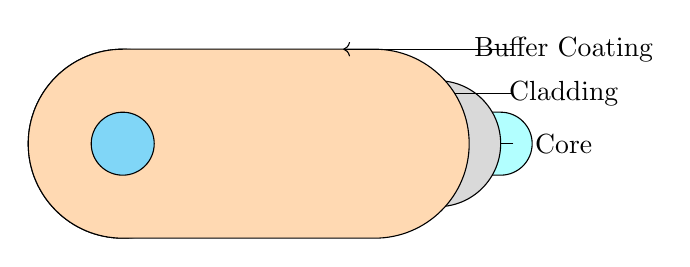
\begin{tikzpicture}[scale=0.8]
    % Core
    \draw[fill=cyan!30] (0,0) ellipse (0.5 and 0.5);
    \draw[top color=cyan!30, bottom color=cyan!30] (0,0.5) -- (6,0.5) arc(90:-90:0.5 and 0.5) -- (0,-0.5) arc(-90:-270:0.5 and 0.5);
    \node at (7,0) {Core};
    \draw[->] (6.2,0) -- (5.5,0);

    % Cladding
    \draw[fill=gray!30] (0,0) ellipse (1 and 1);
    \draw[top color=gray!30, bottom color=gray!30] (0,1) -- (5,1) arc(90:-90:1 and 1) -- (0,-1) arc(-90:-270:1 and 1);
    \node at (7,0.8) {Cladding};
    \draw[->] (6.2,0.8) -- (4.5,0.8);

    % Coating/Buffer
    \draw[fill=orange!30] (0,0) ellipse (1.5 and 1.5);
    \draw[top color=orange!30, bottom color=orange!30] (0,1.5) -- (4,1.5) arc(90:-90:1.5 and 1.5) -- (0,-1.5) arc(-90:-270:1.5 and 1.5);
    \node at (7,1.5) {Buffer Coating};
    \draw[->] (6.2,1.5) -- (3.5,1.5);
    
    % Core visible at front
    \draw[fill=cyan!50] (0,0) ellipse (0.5 and 0.5);
\end{tikzpicture}
\captionof{figure}{Fiber Optic Cable Construction}
\end{center}

\textbf{Main Components:}
\begin{itemize}
    \item \textbf{Core}:
    \begin{itemize}
        \item Central part where light travels
        \item Made of pure silica/glass
        \item High refractive index ($n_1$)
    \end{itemize}
    \item \textbf{Cladding}:
    \begin{itemize}
        \item Surrounds the core
        \item Lower refractive index than core ($n_2 < n_1$)
        \item Reflects light back into core (TIR)
    \end{itemize}
    \item \textbf{Buffer/Jacket}:
    \begin{itemize}
        \item Protective plastic covering
        \item Protects from physical damage and moisture
    \end{itemize}
\end{itemize}
\end{solutionbox}

\begin{mnemonicbox}
"CCB" - "Core, Cladding, Buffer"
\end{mnemonicbox}

\questionmarks{5(c)}{7}{Draw Block Diagram of optical fiber communication and Explain.}

\begin{solutionbox}
\textbf{Answer}:

\begin{center}
\begin{tikzpicture}[node distance=2.2cm, auto, >=latex, thick, scale=0.9, transform shape]
    \node [gtu block] (info) {Info\\Source};
    \node [gtu block, right of=info] (tx) {Electrical\\TX};
    \node [gtu block, right of=tx] (source) {Optical\\Source (LED/Laser)};
    \node [gtu block, right of=source, node distance=3cm] (cable) {Optical\\Fiber Cable};
    \node [gtu block, right of=cable, node distance=3cm] (det) {Optical\\Detector (Diode)};
    \node [gtu block, right of=det] (rx) {Electrical\\RX};
    
    \draw [gtu arrow] (info) -- (tx);
    \draw [gtu arrow] (tx) -- (source);
    \draw [gtu arrow] (source) -- node {Light} (cable);
    \draw [gtu arrow] (cable) -- node {Light} (det);
    \draw [gtu arrow] (det) -- (rx);
\end{tikzpicture}
\captionof{figure}{Optical Fiber Communication}
\end{center}

\textbf{Operation:}
\begin{itemize}
    \item \textbf{Electrical TX}: Encodes input signal into drive current
    \item \textbf{Optical Source}: Converts electrical signal to light pulses (E/O conversion)
    \item \textbf{Optical Fiber}: Carries light via Total Internal Reflection
    \item \textbf{Optical Detector}: Converts light back to electrical signal (O/E conversion) (e.g., Photodiode)
    \item \textbf{Electrical RX}: Amplifies and shapes signal
\end{itemize}

\textbf{Advantages}: High bandwidth, low loss, immune to EMI.
\end{solutionbox}

\begin{mnemonicbox}
"ET-OS-Cable-OD-ER" - "Electrical TX, Optical Source, Cable, Optical Detector, Electrical RX"
\end{mnemonicbox}

\questionmarks{5(a) OR}{3}{Explain Numerical Aperture.}

\begin{solutionbox}
\textbf{Answer}:

\textbf{Numerical Aperture (NA)}: Measure of light-gathering ability of an optical fiber.

\begin{itemize}
    \item It is the sine of the acceptance angle ($\theta_a$) of the fiber
    \item Formula: $NA = \sin \theta_a = \sqrt{n_1^2 - n_2^2}$
    \item Where $n_1$ = core refractive index, $n_2$ = cladding refractive index
    \item Higher NA means more light gathering capability
\end{itemize}

\begin{center}
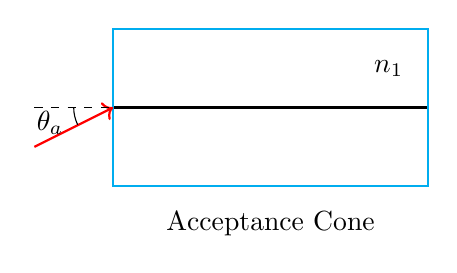
\begin{tikzpicture}[scale=1]
    \draw[thick] (0,0) -- (4,0); % Axis
    \draw[thick, cyan] (0,-1) rectangle (4,1); % Fiber
    \node at (3.5,0.5) {$n_1$};
    
    \draw[->, thick, red] (-1, -0.5) -- (0,0); % Ray
    \draw[dashed] (-1,0) -- (0,0);
    \draw (-0.5,0) arc(180:206:0.5);
    \node at (-0.8, -0.2) {$\theta_a$};
    
    \node[below] at (2,-1.2) {Acceptance Cone};
\end{tikzpicture}
\end{center}
\end{solutionbox}

\begin{mnemonicbox}
"No Sign Theta" - "NA = sin(theta)"
\end{mnemonicbox}

\questionmarks{5(b) OR}{4}{Explain PWM generation and demodulation.}

\begin{solutionbox}
\textbf{Answer}:

\textbf{PWM Generation:}
\begin{itemize}
    \item Generated using a comparator
    \item Sine wave (message) is compared with a sawtooth wave
    \item When Message > Sawtooth $\rightarrow$ Output High
    \item When Message < Sawtooth $\rightarrow$ Output Low
\end{itemize}

\textbf{PWM Demodulation:}
\begin{itemize}
    \item Simple method: Pass PWM signal to an integrator circuit
    \item Integrator produces voltage proportional to pulse width
    \item Follow with Low Pass Filter to smooth signal
\end{itemize}

\begin{center}
\begin{tikzpicture}[auto, >=latex, thick]
    \node (pwm) {PWM};
    \node [gtu block, right of=pwm, node distance=2.5cm] (int) {Integrator};
    \node [gtu block, right of=int, node distance=2.5cm] (lpf) {LPF};
    \node [right of=lpf, node distance=2cm] (out) {Output};
    
    \draw [gtu arrow] (pwm) -- (int);
    \draw [gtu arrow] (int) -- (lpf);
    \draw [gtu arrow] (lpf) -- (out);
\end{tikzpicture}
\captionof{figure}{PWM Demodulator}
\end{center}
\end{solutionbox}

\begin{mnemonicbox}
"Gen Compare, Demod Integrate"
\end{mnemonicbox}

\questionmarks{5(c) OR}{7}{Draw Block Diagram of satellite communication and Explain.}

\begin{solutionbox}
\textbf{Answer}:

\begin{center}
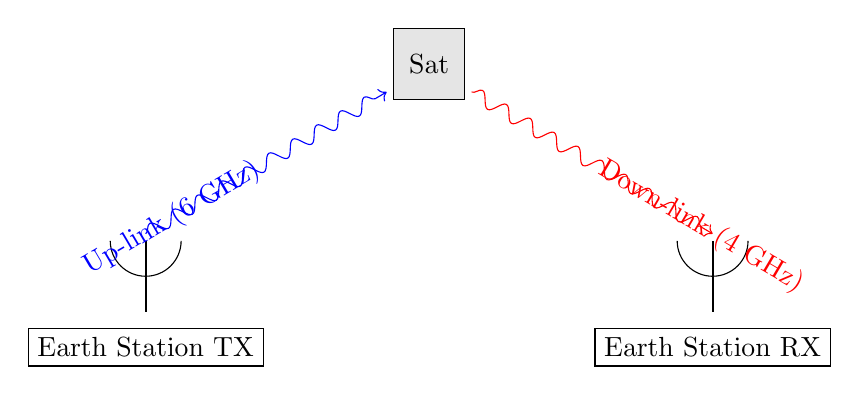
\begin{tikzpicture}[scale=0.9]
    % Earth Station TX
    \node[draw, rectangle] (tx) at (0,0) {Earth Station TX};
    \draw[thick] (0,0.5) -- (0,1.5);
    \draw (-0.5,1.5) arc(180:360:0.5); % Dish
    
    % Satellite
    % Replaced missing image with a drawing
    \node at (4,4) (sat) {}; 
    \draw[fill=gray!20] (3.5,3.5) rectangle (4.5,4.5);
    \node at (4,4) {Sat};
    
    % Earth Station RX
    \node[draw, rectangle] (rx) at (8,0) {Earth Station RX};
    \draw[thick] (8,0.5) -- (8,1.5);
    \draw (7.5,1.5) arc(180:360:0.5); % Dish
    
    % Up-link
    \draw[->, blue, decorate, decoration={snake}] (0,1.6) -- node[left,sloped] {Up-link (6 GHz)} (3.4,3.6);
    
    % Down-link
    \draw[->, red, decorate, decoration={snake}] (4.6,3.6) -- node[right,sloped] {Down-link (4 GHz)} (8,1.6);
    
\end{tikzpicture}
\captionof{figure}{Satellite Communication}
\end{center}

\textbf{Components:}
\begin{enumerate}
    \item \textbf{Earth Station (TX)}: Transmits high power signal to sky (Up-link)
    \item \textbf{Satellite (Transponder)}:
    \begin{itemize}
        \item Receives signal
        \item Changes frequency (Up-link $\rightarrow$ Down-link)
        \item Amplifies signal
        \item Retransmits to earth
    \end{itemize}
    \item \textbf{Earth Station (RX)}: Receives weak signal and processes it (Down-link)
\end{enumerate}

\textbf{Frequencies:} Up-link frequency is always higher than Down-link frequency (e.g. 6/4 GHz).
\end{solutionbox}

\begin{mnemonicbox}
"Up High, Down Low" - Up freq higher, Down freq lower
\end{mnemonicbox}

\end{document}



